\section{Auswertung}
\label{sec:Auswertung}

\subsection{Zeitkonstante eines RC-Kreises} % (fold)
\label{sub:Zeitkonstante}

% subsection Zeitkonstante  (end)

\subsection{Frequenzabhängige Amplitude und Phasenverschiebung} % (fold)
\label{sub:Freque-A&P}

% subsection Frequenzabhängige Amplitude und Phasenverschiebung (end)

\subsection{Ein RC-Kreis als Integrator} % (fold)
\label{sub:Integrator}

% subsection Ein RC-Kreis eines Integrators (end)
\begin{figure}
  \centering
  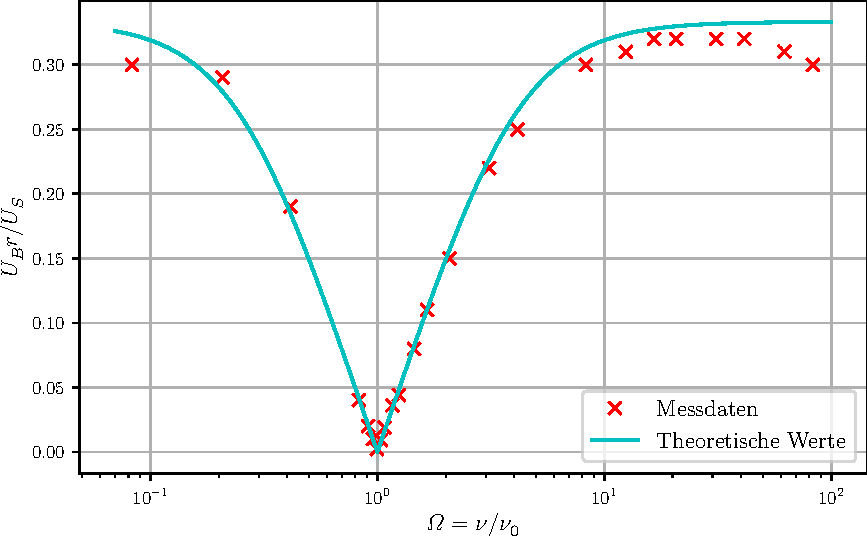
\includegraphics{plot.pdf}
  \caption{Plot.}
  \label{fig:plot}
\end{figure}


Siehe \autoref{fig:plot}!
